\documentclass[letterpaper]{article}
\usepackage{amsmath}
\usepackage{geometry}
\usepackage[utf8]{inputenc}
\usepackage{listings}
\usepackage{hyperref}
\usepackage{xcolor}
\usepackage[shortlabels]{enumitem}
\usepackage[skip=12pt, indent=0pt]{parskip}
\usepackage{makecell}
\usepackage{tablefootnote}
\usepackage{graphicx}


\geometry{letterpaper,left=1in,right=1in,top=1.0in,bottom=1.0in,headheight=28pt}

\definecolor{codegreen}{rgb}{0,0.6,0}
\definecolor{codegray}{rgb}{0.5,0.5,0.5}
\definecolor{codecrimson}{RGB}{153,0,0}
\definecolor{backcolour}{rgb}{0.95,0.95,0.92}
\makeatletter
\lstdefinestyle{mystyle}{
  backgroundcolor=\color{backcolour},   commentstyle=\color{codegreen},
  keywordstyle=\color{blue},
  numberstyle=\tiny\color{codegray},
  stringstyle=\color{codecrimson},
  basicstyle=\ttfamily,
  breakatwhitespace=false,         
  breaklines=true,                 
  captionpos=b,                    
  keepspaces=true,                 
  numbers=left,                    
  numbersep=5pt,                  
  showspaces=false,                
  showstringspaces=false,
  showtabs=false,                  
  tabsize=2
}
\makeatother
\lstset{style=mystyle}

\renewcommand{\year}{2026}

\title{Lab 05 - Krylov Methods and PETSc}
\author{Kabelo Tsiane}
\date{October 2nd \year}
\newcommand{\duedate}{October 16th \year -- 11:58 pm\\ (Two minutes to midnight)}

\begin{document}

\maketitle

\begin{center}
    NERS/ENGR 570 Fall \year \\
    DUE BY: \duedate \\
\end{center}

%\section*{Learning Objectives}

\section*{Exercise 1 (25 pts) -- Install PETSc}

In this exercise you are to download, configure, build, test your build, and install PETSc.
The purpose of this exercise is to assess how well you have learned the material presented in Lectures 4-5, and Labs 1-4.
Your subsequent PETSc installation will be used for the remaining exercises.

\textbf{For your PETSc \underline{installation}, use your class directory space located at:}\\
\lstinline{/gpfs/accounts/ners570f26_class_root/ners570f26_class/\$USER}

\begin{enumerate}
    \item Download PETSc. What command did you use? \\

    git clone -b release https://gitlab.com/petsc/petsc.git petsc \\
    git pull
    
    \item Load any modules you think would be prerequisites for PETSc. Document your loaded modules at configure-time. \\
\begin{lstlisting}
    (base) [kabelo@gl-login5 tutorials]$ module list

    Currently Loaded Modules:
        1) gcc/15.1.0   2) openmpi/5.0.10   3) openblas/0.3.30
    \end{lstlisting}
    \item The next step is to configure PETSc.
    \begin{itemize}
        \item Since you wish to use PETSc--rather than contribute source to it-- you desire your library installation to run as fast as possible. \\
        \\
        I use the option \texttt{--with-debugging=0}
        \item You also wish to \textbf{include debug symbols} in case you develop against the library incorrectly.
        I use the option \texttt{--COPTFLAGS="-O3 -g"} where -g is for the debug symbols.
        \item What command did you use to configure PETSc? 
    \end{itemize}
\begin{lstlisting}
    ./configure --with-openblas-dir=/sw/pkgs/arc/stacks/gcc/15.1.0/OpenBLAS/0.3.30\\
    --with-mpi-dir=/sw/pkgs/arc/stacks/gcc/15.1.0/openmpi/5.0.10\\
    --prefix=/gpfs/accounts/ners570f26\_class\_root/ners570f26\_class/kabelo/petsc\\
    --with-debugging=0 --COPTFLAGS="-O3 -g" 
\end{lstlisting}
    \item Check the build to verify correctness by running tests. What command did you use? Did any checks or tests fail? If so, which ones? \\
    All checks passed when I ran:
\begin{lstlisting}
    make PETSC_DIR=/gpfs/accounts/ners570f26_class_root/ners570f26_class/kabelo/petsc PETSC_ARCH="" check
\end{lstlisting}
    \item Install your PETSc build. What command did you use? \\
\begin{lstlisting}
    make PETSC_DIR=/home/kabelo/petsc PETSC_ARCH=arch-linux-c-opt install
\end{lstlisting}
    \item In the following exercises you will be working with PETSc’s tutorial example 15. The tutorial is provided in both C and Fortran.
        Source code for the example can be viewed at the links below.\\
        \url{https://petsc.org/release/src/ksp/ksp/tutorials/ex15.c.html}\\
        \url{https://petsc.org/release/src/ksp/ksp/tutorials/ex15f.F90.html}

    \item Read through the source file and provide a written summary in your own words of what the program does. Do not use LLMs or GenAI for this part. \\

    This program solves a linear system using parallel Krylov Methods. It allows the user to use pre-existing preconditioners, as well as user-defined preconditioners to use in solving the linear system. It computes the matrix and right-hand-side vector that define the linear system, $A\mathbf{x} = b$. It creates the linear solver and sets various options including the preconditioner, $P$, and its relevant routines. Finally it solves the linear system, checks the solution and does some cleanup.
    
    \item Fortunately for you, the example we’ll be working with is installed!
        Can you find the source file in your install directory? Where did you find the example/tutorial?
\begin{lstlisting}
find ./ -name *ex15.c
\end{lstlisting}
        Using the above command from the petsc install root, I found the example in:\\ \texttt{./share/petsc/examples/src/ksp/ksp/tutorials}
        \\
        To compile the example, go to the directory with the file.
        In this directory you should run \lstinline{make} with the appropriate make options and target name for the example you want to work with (C or Fortran).
\begin{lstlisting}
make PETSC_DIR=/gpfs/accounts/ners570f26_class_root/ners570f26_class/kabelo/petsc ex15
\end{lstlisting}
    \item Additional notes for the next exercises
    \begin{itemize}
        \item If you modify the source, run \lstinline{make clean} before you run \lstinline{make} to ensure that your previous compilations do not affect your latter compilation.
        \item You will be running an MPI executable in parallel for this assignment (and we have not covered this in detail in lecture yet).\
            So here is the base command you will use:
\begin{lstlisting}
$ mpiexec -np <numprocs> [<path to executable>/]<exename>
\end{lstlisting}
            To  report times use the “real” time reported by the time command e.g.
\begin{lstlisting}
$ time mpiexec -np <numprocs> [<path to executable>/]<exename>
\end{lstlisting}
            For the various cases you will run, many of the options can be controlled from the command line. Some of the useful command line options are:
            \begin{itemize}
                \item \lstinline{-ksp_type}
                \item \lstinline{-pc_type}
                \item \lstinline{-mat_view ascii}
                \item \lstinline{-log_view}
                \item \lstinline{-ksp_monitor}
            \end{itemize}

            For more information, see PETSc’s documentation (see the section on \href{https://petsc.org/release/manual/ksp/#}{Krylov Solvers}) for this assignment (\url{https://petsc.org/release/docs/manual}).
            Try to use \lstinline{-log_view} and interpret the output information to help understand the meaning of the options provided.

        \item The matrix size can also be changed using command line options.
            In this example, the matrix is set from a 2-D five-point stencil for a $m$ by $n$ rectangular grid with $m \times n$ unknowns, so $A$ is always a square matrix of size $m \times n$.
            To change the values of $m$ or $n$, use the intuitive command line options \lstinline{-n} and \lstinline{-m}
    \end{itemize}
\end{enumerate}


\underline{\textit{Extra-credit (5 pts)}}\\
Write a module file for your PETSc install. \\

\begin{lstlisting}
    -- petsc/3.26.lua

    whatis([[ This package runs the Portable Extensible Toolkit for Scientific Computing.
            It exists to run ex15 tutorial exercise as a part of NERS570FA26. ]])

    depends_on("gcc/15.1.0", "openmpi/5.0.10")
    local root = "/gpfs/accounts/ners570f26_class_root/ners570f26_class/kabelo/petsc"
    setenv("PETSC_DIR", root)
    prepend_path("LD_LIBRARY_PATH", pathJoin(root, "lib"))
\end{lstlisting}

\underline{\textit{Extra-credit (2 pts)}}\\
Determine the compile and link commands for \lstinline{ex15} without using the PETSc Makefile.

I just ran \texttt{make -n ex15} and got this:
\begin{lstlisting}
/sw/pkgs/arc/stacks/gcc/15.1.0/openmpi/5.0.10/bin/mpicc -o  ex15.o -c -fPIC -Wall -Wwrite-strings -Wno-unknown-pragmas -Wno-lto-type-mismatch -Wno-stringop-overflow -fstack-protector -fvisibility=hidden -O3 -g  -I/gpfs/accounts/ners570f26_class_root/ners570f26_class/kabelo/petsc/include -I/sw/pkgs/arc/stacks/gcc/15.1.0/OpenBLAS/0.3.30/include -I/sw/pkgs/arc/stacks/gcc/15.1.0/openmpi/5.0.10/include    ex15.c
/sw/pkgs/arc/stacks/gcc/15.1.0/openmpi/5.0.10/bin/mpicc -fPIC -Wall -Wwrite-strings -Wno-unknown-pragmas -Wno-lto-type-mismatch -Wno-stringop-overflow -fstack-protector -fvisibility=hidden -O3 -g  -I/gpfs/accounts/ners570f26_class_root/ners570f26_class/kabelo/petsc/include -I/sw/pkgs/arc/stacks/gcc/15.1.0/OpenBLAS/0.3.30/include -I/sw/pkgs/arc/stacks/gcc/15.1.0/openmpi/5.0.10/include     -Wl,-export-dynamic -o ex15 ex15.o    -Wl,-rpath,/gpfs/accounts/ners570f26_class_root/ners570f26_class/kabelo/petsc/lib -L/gpfs/accounts/ners570f26_class_root/ners570f26_class/kabelo/petsc/lib -Wl,-rpath,/sw/pkgs/arc/stacks/gcc/15.1.0/OpenBLAS/0.3.30/lib -L/sw/pkgs/arc/stacks/gcc/15.1.0/OpenBLAS/0.3.30/lib -Wl,-rpath,/sw/pkgs/arc/stacks/gcc/15.1.0/openmpi/5.0.10/lib -L/sw/pkgs/arc/stacks/gcc/15.1.0/openmpi/5.0.10/lib -Wl,-rpath,/sw/pkgs/arc/gcc/15.1.0/lib64 -L/sw/pkgs/arc/gcc/15.1.0/lib64 -Wl,-rpath,/sw/pkgs/arc/gcc/15.1.0/lib/gcc/x86_64-pc-linux-gnu/15.1.0 -L/sw/pkgs/arc/gcc/15.1.0/lib/gcc/x86_64-pc-linux-gnu/15.1.0 -Wl,-rpath,/sw/pkgs/arc/gcc/15.1.0/lib -L/sw/pkgs/arc/gcc/15.1.0/lib -lpetsc -lopenblas -lm -lX11 -ldl -lmpi_usempif08 -lmpi_usempi_ignore_tkr -lmpi_mpifh -lmpi -lgfortran -lm -lgfortran -lm -lgcc_s -lquadmath -lpthread -lstdc++ -lquadmath -ldl 
\end{lstlisting}

\clearpage

\section*{Exercise 2 (35 pts) -- Comparison of Krylov Methods}
In lecture 09 and Lab 05 we covered Krylov methods and showed you some comparisons using a Jupyter notebook.
In this exercise we will compare the different Krylov methods as they are implemented in PETSc.
Be sure to exclude any preconditioning by using the \lstinline{-pc_type none option}.

\begin{table}[h!]
    \centering
    \caption{Number of Iterations and runtime}
    \begin{tabular}{|c|c|c|c|c|c|c|}
    \hline
     Grid Size & CG & BiCGSTAB & \thead{GMRES\\ (no restart\tablefootnote{Let PETSc build the subspace for GMRES up to the maximum iterations (10,000)})} & \thead{GMRES\\ (restart=30)} & \thead{GMRES\\ (restart=200)} \\\hline
     $m=n=8$    & \thead{10\\(00:00:11.859)}   & \thead{10\\(00:00:00.369)}   & \thead{10\\(00:00:06.806)}   & \thead{10\\(00:00:00.387)}                     & \thead{10\\(00:00:00.396)}   \\\hline
     $m=n=32$   & \thead{58\\(00:00:00.423)}   & \thead{44\\(00:00:00.378)}   & \thead{58\\(00:00:01.333)}   & \thead{119\\(00:00:00.384)}                    & \thead{58\\(00:00:00.366)}   \\\hline
     $m=n=128$  & \thead{218\\(00:00:00.428)}  & \thead{168\\(00:00:00.413)}  & \thead{214\\(00:00:01.728)}  & \thead{1341\\(00:00:00.797)}                   & \thead{216\\(00:00:00.674)}  \\\hline
     $m=n=256$  & \thead{427\\(00:00:00.649)}  & \thead{326\\(00:00:00.783)}  & \thead{415\\(00:00:09.008)}  & \thead{4501\\(00:00:06.312)}                   & \thead{753\\(00:00:06.518)}  \\\hline
     $m=n=512$  & \thead{838\\(00:00:02.648)}  & \thead{603\\(00:00:03.689)}  & \thead{801\\(00:01:52.406)}  & \thead{10000\textsuperscript{\dag}\\(00:01:11.058)} & \thead{2489\\(00:01:32.951)} \\\hline
     $m=n=1024$ & \thead{1637\\(00:00:23.029)} & \thead{1116\\(00:00:31.639)} & \thead{1543\\(00:32:44.237)} & \thead{10000\textsuperscript{\dag}\\(00:05:41.039)} & \thead{8888\\(00:23:32.722)} \\\hline
    \end{tabular}

    \vspace{4pt}
    {\footnotesize \textsuperscript{\dag}Did not converge: reached the maximum of 10,000 iterations (\texttt{DIVERGED\_ITS}).}
\end{table}


Discuss the observed results in several sentences.
Which method scaled best with grid size?
How did the number of restart vectors affect the number of iterations? \\

CG scaled the best with grid size. A 32 x 32 grid took 0.423s to converge, this rose to 23s for a 1024 x 1024 grid. Every other method took longer to converge for the 1024 x 1024 grid, from 31s for BICGSTAB to several minutes for the rest even though they all took less than 2s for the 32 x 32 grid. \\
Having smaller restarts led to an increased number of iterations for GMRES, this is because fewer restart vectors means the solver must iterate more frequently to converge. More iterations but less memory intensive.

Hint: the different Krylov methods may be chosen with a command line option.
The keyword and options are in the User's manual.

\underline{\textit{Extra-credit (5 pts)}}\\
Extend the analysis and evaluate flexible and pipelined variants of GMRES

\underline{\textit{Extra-credit (5 pts)}}\\
Extend the analysis and evaluate the flexible and improved variants of BiCGSTAB

\clearpage
\section*{Exercise 3 (40 pts) -- Preconditioners}
In Lab 05 and Lecture 09 we covered Krylov methods and spent some time discussing how they converge and that this was related to the condition number.
We also mentioned that matrices resulting from typical finite difference discretizations have an unbounded condition number as the problem size increases.
This means that Krylov methods may struggle for large problems without a preconditioner.
The purpose of this exercise is to observe how preconditioners can help this situation.

In this exercise we ask you to perform an experimental analysis using PETSc and look at the effectiveness of various preconditioners, both in terms of performance and ability to reduce the original matrix’s condition number.

\subsection*{Part A -- Preconditioner Performance}
Fill in the following table and discuss the results.
When running your calculations to get timing info, be sure to suppress extraneous output (e.g. \lstinline{-log_view}, \lstinline{-mat_view}, etc.) and run on the compute nodes.
\textbf{USE 1 PROCESSOR AND THE DEFAULT RESTART LENGTH HERE.}

\begin{table}[h!]
    \centering
    \caption{Number of GMRES Iterations and runtime}
    \begin{tabular}{|c|c|c|c|c|c|}
    \hline
     Grid Size & Jacobi & SOR & \thead{Incomplete\\ LU} & \thead{Incomplete\\ Cholesky} & \thead{Algebraic\\ Multigrid} \\\hline
     $m=n=8$    & \thead{10\\(00:00:04.876)}                     & \thead{10\\(00:00:00.364)}   & \thead{9\\(00:00:00.366)}    & \thead{9\\(00:00:00.372)}    & \thead{7\\(00:00:00.383)}  \\\hline
     $m=n=32$   & \thead{119\\(00:00:00.372)}                    & \thead{32\\(00:00:00.345)}   & \thead{27\\(00:00:00.324)}   & \thead{27\\(00:00:00.339)}   & \thead{8\\(00:00:00.327)}  \\\hline
     $m=n=128$  & \thead{1341\\(00:00:00.796)}                   & \thead{167\\(00:00:00.433)}  & \thead{119\\(00:00:00.394)}  & \thead{119\\(00:00:00.395)}  & \thead{8\\(00:00:00.374)}  \\\hline
     $m=n=256$  & \thead{4501\\(00:00:07.444)}                   & \thead{590\\(00:00:01.813)}  & \thead{454\\(00:00:01.374)}  & \thead{454\\(00:00:01.354)}  & \thead{9\\(00:00:00.522)}  \\\hline
     $m=n=512$  & \thead{10000\textsuperscript{\dag}\\(00:01:15.860)} & \thead{2176\\(00:00:25.499)} & \thead{1636\\(00:00:16.488)} & \thead{1636\\(00:00:16.872)} & \thead{10\\(00:00:01.368)} \\\hline
     $m=n=1024$ & \thead{10000\textsuperscript{\dag}\\(00:05:31.652)} & \thead{7376\\(00:05:59.453)} & \thead{5555\\(00:03:54.017)} & \thead{5555\\(00:03:58.166)} & \thead{11\\(00:00:05.705)} \\\hline
    \end{tabular}

    \vspace{4pt}
    {\footnotesize \textsuperscript{\dag}Did not converge: reached the maximum of 10,000 iterations (\texttt{DIVERGED\_ITS}).}
\end{table}


Questions
\begin{enumerate}
    \item What options did you use to run each preconditioner? \\
    
    -pc\_type jacobi ; -pc\_type sor ; -pc\_type ilu ; -pc\_type icc ; -pc\_type gamg
    \item Which preconditioner gave the largest increase in average time per iteration? \\
    
    The default restart time for GMRES is 30, so this column in the table for exerecise 2 is used as the no preconditioner result. For each preconditioner, the average time per iteration is computed across grid sizes. The average time without a preconditioner was 0.0142 s/iteration. The largest increase was found when using the Algebraic Multigrid method, which has average time 0.143 s/iteration. 
    \item Explain the basic mathematics of each preconditioner and how it works. This should include a several sentences and some equations. \\

    Each method tries to solve the following left preconditioned linear system: $$P^{-1}(A\mathbf{x} - \mathbf{b}) = 0$$
    Or equivalently this right preconditioned system: $$AP^{-1}(P\mathbf{x}) = \mathbf{b}$$. This reduces the condition number and increases the rate of convergence. To build the precondition matrix $P$, the methods differ and are broadly split into iterative methods, and (approximate) direct methods: \\
    \textbf{Jacobi}: Let $A = L+D+U$, where $L, U$ are strictly lower and upper triangular respectively, $D$ is the diagonal. Define $T=-D^{-1}(L+U)$ such that each iterative solution looks like $$\mathbf{x}^{(l+1)} = T^{(l)}\mathbf{x}^{(l)} + \mathbf{c}$$The preconditioner $P$ thus chosen looks like $P=\mathrm{diag}(A)$ \\
    \textbf{Incomplete Cholesky}: Define $A = LL^T$ where $L$ is a lower triangular matrix. This is the Cholesky factorization. Incomplete Cholesky factorization constructs a lower triangular matrix $K$ that is sparser than $L$, to prevent fill-in since the factors $L, L^T$ tend too be much less sparse than $A$. Constructed this way, $A \approx KK^T$. The preconditioner $P=KK^T$ \\
    \textbf{Incomplete LU}: Define $A=LU$ where $L$ and $U$ are lower and upper triangular. The $L, U$ factors tend to be less sparse than $A$ so more sparse approximations to $L, U$ are used instead to give $A \approx LU$. The preconditioner $P=LU$. \\
    \textbf{SOR}: A variant of Gauss-Seidel iteration. Let $A=(D+L+U)$. Define relaxation factor $\omega > 1$. Then each solution looks like 
    $$\begin{aligned}
        \mathbf{x}^{(l+1)} &= (D + \omega L)^{-1} \left(\omega \mathbf{b} - [\omega U + (\omega - 1)D]\mathbf{x}^{(l)}\right) \\
        &= T\mathbf{x}^{(l)} + \mathbf{c}, \\
        \\
        \rightarrow T &= -(D + \omega L)^{-1}[\omega U + (\omega - 1)D]
    \end{aligned}$$
    The preconditioner $P=\frac{1}{\omega}(D + \omega L)$. \\
    \textbf{Algebraic Multigrid}: the goal here is to map residual errors from some fine grid to a coarser grid. Steps included are to smooth out high frequency errors using some classical iteration scheme. You need some restriction operator to map errors on the fine grid to the coarse grid. Conversely you need an interpolation operator to do the mapping from the coarse grid to the fine grid, accounting for corrections. There must be a step to add the prolongated coarser grid solution to the finer grid
\end{enumerate}

Create 2 plots.
One for run time vs grid size, and the other for iterations vs grid size.
Discuss the results in a few sentences describing observations and providing explanations for those observations.

\begin{figure}[h!]
    \centering
    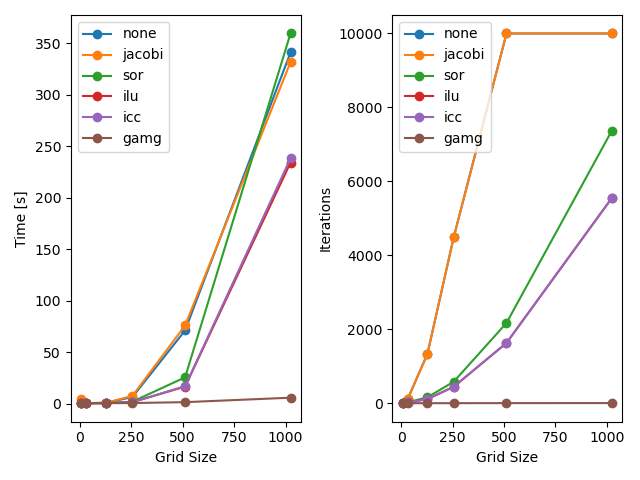
\includegraphics[width=0.5\columnwidth]{ex3.png}
    \caption{Comparing Preconditioned Convergence. \textit{Left}: Grid Size vs Time [s]. \textit{Right}: Grid Size vs Iterations}
    \label{fig:comp}
\end{figure}

The Algebraic Multigrid method is the fastest, with a fairly consistent time and number of iterations till convergence. Performance is so consistent because mapping the errors to different grids occurs in similar number of steps regardless of matrix size. Incomplete Cholesky/LU are next fastest in time to converge, since the direct factorization of the coefficient Matrix is done once. Whereas the iterative methods (Jacobi, SOR) need many iterations to converge. The iterative methods are all comparable to not using a preconditioner, probably because these matrices are not large, and possibly not sparse either. I would expect iterative methods to become faster then the direct methods as the grid size increases. \\

In the grid size vs iterations plot it looks like Incomplete LU/Cholesky finish in identical numbers of iterations. Both take fewer iterations than every iterative method since they are direct solvers.

\clearpage
\subsection*{Part B -- Estimate the Condition Number of Various Grid Sizes}
The condition number can be edited during the GMRES iterations with the appropriate command line options.
These options are not well documented in the manual, but they are documented.
Try doing a bit of searching (especially on the PETSc website) to find the discussion of how to edit condition numbers.
For the condition number estimates, take the maximum value over all iterations.
\textbf{USE 1 PROCESSOR HERE.}

\begin{table}[h!]
    \centering
    \caption{Estimated Condition Number for Various Preconditioners}
    \begin{tabular}{|c|c|c|c|c|c|c|}
    \hline
     Grid Size & None & Jacobi & SOR & \thead{Incomplete\\ LU} & \thead{Incomplete\\ Cholesky} & \thead{Algebraic\\ Multigrid} \\\hline
     $m=n=8$     & 29.28  & 29.28  & 4.864 & 3.617 & 3.617 & 1.439 \\\hline
     $m=n=32$    & 437.7  & 437.7  & 55.97 & 39.68 & 39.68 & 1.732 \\\hline
     $m=n=128$   & 6741   & 6741   & 844.0 & 596.6 & 596.6 & 2.117 \\\hline
     $m=n=256$   & 26765  & 26765  & 3347  & 2366  & 2366  & 2.494 \\\hline
     $m=n=512$   & 106655 & 106655 & 13334 & 9428  & 9428  & 3.284 \\\hline
     $m=n=1024$  & 425798 & 425798 & 53230 & 37636 & 37636 & 4.686 \\\hline
    \end{tabular}
\end{table}


Questions
\begin{enumerate}
    \item Which preconditioner gave the largest reduction in the condition number? \\

    The Algebraic Multigrid gave the a largest reduction in condition number. For $m = n = 1024$ the $\kappa$ drops from 425798 without a preconditioner, to $\kappa = 4.686$ using the Algebraic Multigrid preconditioner.
    
    \item Does this corroborate or contradict the results in Part A comparing the number of iterations? \\

    These findings corroborate what we found in Part A. For a given matrix size, the faster a method converges, the lower its condition number. Furthermore for different methods, a similar condition number gives a similar time to convergence.
\end{enumerate}

\underline{\textit{Extra-credit (5 pts)}}\\
Repeat the calculations for CG without a preconditioner.
Verify that the reduction in error for each iteration adheres to the following expression for rate of convergence of CG for a symmetric positive definite matrix:
\begin{equation*}
    \frac{||e_k||_A}{||e_0||_A} \leq 2 \left( \frac{\sqrt{\kappa}-1}{\sqrt{\kappa}+1} \right)^k
\end{equation*}

\underline{\textit{Extra-credit (5 pts)}}\\
For part A of exercise 3, repeat the study for the preconditioners provided by hypre.
Note you may have to rebuild PETSc with hypre.

\clearpage
\section*{Deliverables and how to submit}
For the overall deliverable you may submit a single word doc or pdf based on these instructions. Name the file as follows:\\
\lstinline{<username>_Lab05.pdf}

For exercise 1, include the commands you executed for each part of the exercise for downloading, configuring, compiling, testing, and installing.

For exercise 2, include 1 sample slurm script that you used.

Include answers for all questions.

Upload your pdf file to canvas.

For extra-credit, include this in your submitted pdf.


\section*{Slurm Script}
Batch script (\texttt{q2.sh}) used to generate the performance results for the various KSP solver configurations.
\begin{lstlisting}[language=bash]
#!/usr/bin/bash
#SBATCH --job-name=q2
#SBATCH --account=ners570f26_class
#SBATCH --nodes=1
#SBATCH --ntasks-per-node=1
#SBATCH --cpus-per-task=1
#SBATCH --mem-per-cpu=90G
#SBATCH --time=02:00:00

module load gcc/15.1.0 openmpi/5.0.10

EXE=/gpfs/accounts/ners570f26_class_root/ners570f26_class/kabelo/petsc/share/petsc/examples/src/ksp/ksp/tutorials/ex15

# GMRES with no restart (restart=10000) runs as its own job in q2_gmres_norestart.sh
for ksp_type in cg bcgs gmres
do
    if [[ $ksp_type == "gmres" ]]; then
        for rstart in 30 200
        do
            for dim in 8 32 128 256 512 1024
            do
                echo -e " ${dim} x ${dim} ${ksp_type} restart = ${rstart}\n"
                time mpiexec -np 1 ${EXE} -pc_type none -m ${dim} -n ${dim} \
                -ksp_type $ksp_type \
                -ksp_max_it 10000 -ksp_gmres_restart $rstart \
                -ksp_converged_reason
                echo
            done
        done
    else
        for dim in 8 32 128 256 512 1024
        do
            echo -e " ${dim} x ${dim} ${ksp_type}\n"
            time mpiexec -np 1 ${EXE} -pc_type none -m ${dim} -n ${dim} \
            -ksp_type $ksp_type \
            -ksp_converged_reason
            echo
        done
    fi
done > q2_timing.txt 2>&1
\end{lstlisting}

\end{document}
